% Intended LaTeX compiler: xelatex
\documentclass[12pt]{spbstu-task}
\usepackage{graphicx}
\usepackage{float}
\usepackage{booktabs}
\usepackage{dsfont}
\usepackage{hyperref}
\setmainfont{Times New Roman}
\defaultfontfeatures{Ligatures=TeX,Scale=MatchLowercase,Mapping=tex-text}
\hypersetup{hidelinks}
\allowdisplaybreaks
\captionsetup[table]{labelsep=period}
\captionsetup[figure]{labelsep=period}
\setlength{\abovecaptionskip}{5pt}
\setlength{\belowcaptionskip}{0pt}
\newcommand{\E}{\mathbb{E}}
\newcommand{\D}{\mathbb{D}}
\renewcommand{\Prob}{\mathbf{P}}
\newcommand{\ind}{\mathds{1}}
\DeclareMathOperator{\Bias}{Bias}
\begin{document}

\sloppy
\pagenumbering{arabic}

\noindent\textbf{Салимли Айзек Мухтар оглы}\hfill\textbf{гр. 5140201/60301}

\begin{center}
  \textbf{ИДЗ №2 (Классическая статистика)}\\[0.4em]
  \textbf{Вариант 16}
\end{center}

\noindent\textbf{Задание:}

\begin{center}
  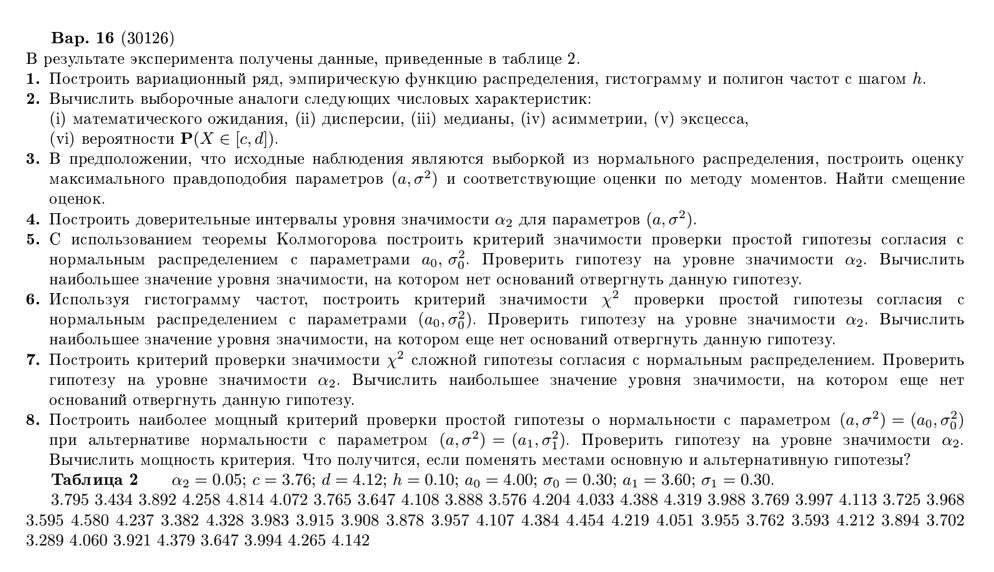
\includegraphics[width=\textwidth]{fig/task.png}
\end{center}

%% Пункт 1
\subsection*{1. Вариационный ряд, эмпирическая функция распределения, гистограмма и полигон частот}

\textbf{Вариационный ряд} \(x_{(1)} \le x_{(2)} \le \ldots \le x_{(50)}\):

{\small
\noindent 3.289, 3.382, 3.434, 3.576, 3.593, 3.595, 3.647, 3.647, 3.702, 3.725, 3.762, 3.765, 3.769,
3.795, 3.878, 3.888, 3.892, 3.894, 3.908, 3.915, 3.921, 3.955, 3.957, 3.968, 3.983, 3.988, 3.994,
3.997, 4.033, 4.051, 4.060, 4.072, 4.107, 4.108, 4.113, 4.142, 4.204, 4.212, 4.219, 4.237, 4.258,
4.265, 4.319, 4.328, 4.379, 4.384, 4.388, 4.454, 4.580, 4.814.
\par}

\textbf{Эмпирическая функция распределения:}
\begin{displaymath}
  F_n(x) = \frac{1}{n}\sum_{i=1}^{n}\ind\{X_i \le x\} =
  \begin{cases}
    0, & x < x_{(1)},\\
    \dfrac{j}{n}, & x_{(j)} \le x < x_{(j+1)},\\
    1, & x \ge x_{(n)}.
  \end{cases}
\end{displaymath}
Функция ступенчатая, в каждой точке \(x_{(j)}\) скачок \(1/n = 0.02\)
(в точке 3.647 значение встречается дважды, скачок \(2/n\)).

\begin{center}
  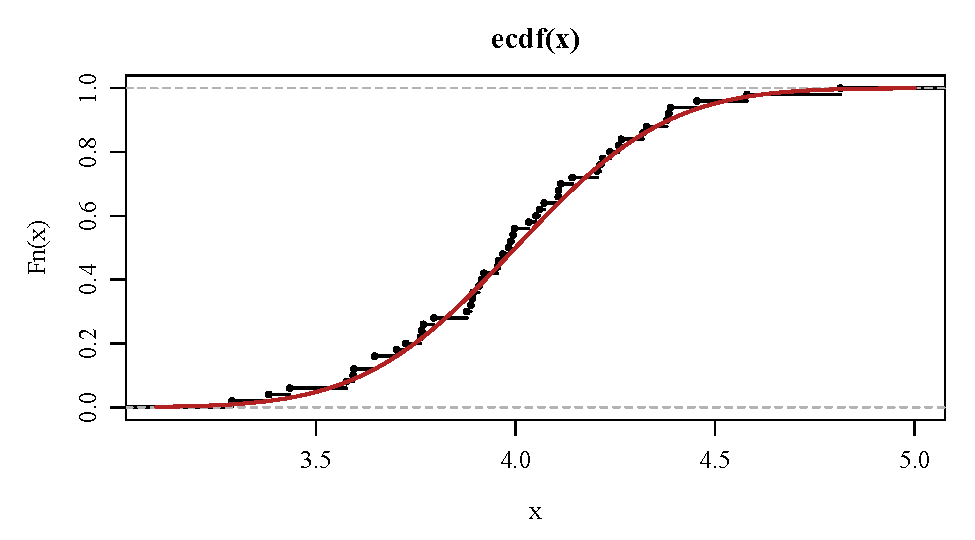
\includegraphics[width=0.92\textwidth]{fig/t1_ecdf.pdf}
\end{center}

\textbf{Группировка с шагом \(h = 0.1\).} Интервалы \((l_i, l_i + h]\), \(l_1 = 3.2\), последний
\((4.8, 4.9]\), всего 17 интервалов; \(\nu_i\) - число наблюдений в интервале.

\begin{table}[H]
  \caption{Группированный ряд}
  \centering
  \small
  \begin{tabularx}{\textwidth}{l*{9}{Y}}
    \toprule
    \(l_i\): левая граница & 3.2 & 3.3 & 3.4 & 3.5 & 3.6 & 3.7 & 3.8 & 3.9 & 4.0 \\
    \(\nu_i\): частота & 1 & 1 & 1 & 3 & 2 & 6 & 4 & 10 & 4 \\
    \(\nu_i/(nh)\): высота столбца & 0.2 & 0.2 & 0.2 & 0.6 & 0.4 & 1.2 & 0.8 & 2.0 & 0.8 \\
    \midrule
    \(l_i\): левая граница & 4.1 & 4.2 & 4.3 & 4.4 & 4.5 & 4.6 & 4.7 & 4.8 & \\
    \(\nu_i\): частота & 4 & 6 & 5 & 1 & 1 & 0 & 0 & 1 & \\
    \(\nu_i/(nh)\): высота столбца & 0.8 & 1.2 & 1.0 & 0.2 & 0.2 & 0 & 0 & 0.2 & \\
    \bottomrule
  \end{tabularx}
\end{table}

\textbf{Гистограмма:} над каждым интервалом прямоугольник высоты \(\nu_i/(nh)\), тогда его площадь
равна относительной частоте \(\nu_i/n\), а общая площадь равна 1, поэтому гистограмму можно сравнивать
с плотностью. \textbf{Полигон частот:} ломаная через точки \(\left(l_i + \frac{h}{2},\ \frac{\nu_i}{nh}\right)\),
замкнутая на ось в серединах соседних пустых интервалов.

\begin{center}
  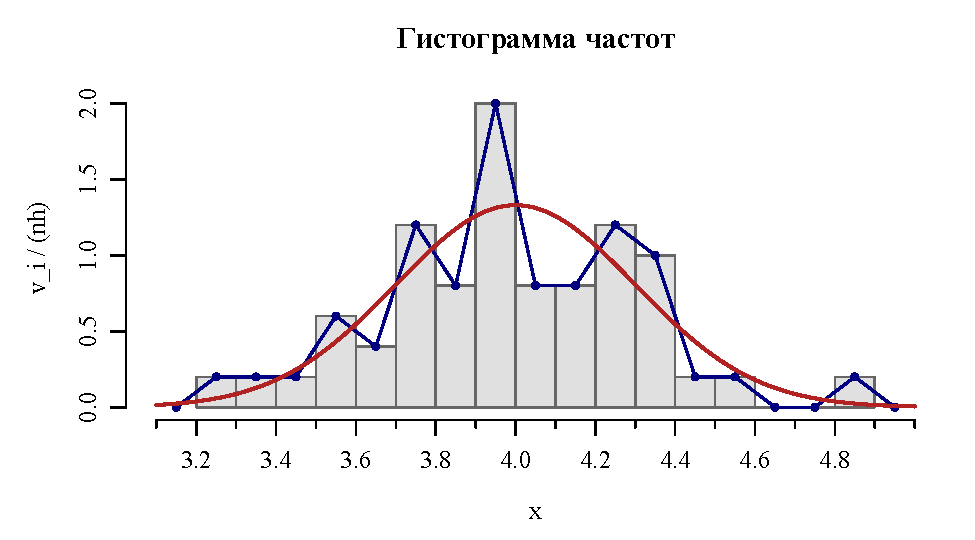
\includegraphics[width=0.92\textwidth]{fig/t1_hist.pdf}
\end{center}

Почти симметрично относительно 4, близко к нормальному визуально.

%% Пункт 2
\subsection*{2. Выборочные аналоги числовых характеристик}
\begin{itemize}[label=\textbullet]
  \item \textbf{Математическое ожидание:} \(\bar{X}\) - выборочное среднее,
  \begin{displaymath}
    \bar{X} = \frac{1}{n}\sum_{i=1}^{n}X_i = \frac{199.546}{50} = 3.99092.
  \end{displaymath}
  \item \textbf{Дисперсия:} \(s^2\) - выборочная дисперсия, \(s = \sqrt{s^2}\) - выборочное стандартное отклонение,
  \begin{gather*}
    s^2 = \frac{1}{n}\sum_{i=1}^{n}\left(X_i - \bar{X}\right)^2 = \frac{1}{n}\sum_{i=1}^{n}X_i^2 - \bar{X}^2 =\\
    = \frac{801.035884}{50} - 3.99092^2 = 0.093275,\qquad s = 0.30541.
  \end{gather*}
  \item \textbf{Медиана:} \(\tilde{X}\) - выборочная медиана, при четном \(n = 50\) полусумма двух средних членов
  вариационного ряда,
  \begin{displaymath}
    \tilde{X} = \frac{x_{(25)} + x_{(26)}}{2} = \frac{3.983 + 3.988}{2} = 3.9855.
  \end{displaymath}
  \item \textbf{Асимметрия и эксцесс:} \(\hat{\gamma}_1\) - выборочный коэффициент асимметрии,
  \(\hat{\gamma}_2\) - выборочный коэффициент эксцесса. Они выражаются через выборочные центральные моменты
  \(m_k = \frac{1}{n}\sum_{i=1}^{n}\left(X_i - \bar{X}\right)^k\) (\(m_3\) - третий, \(m_4\) - четвертый)
  и степени стандартного отклонения \(s^3 = \left(s^2\right)^{3/2}\), \(s^4 = \left(s^2\right)^2\):
  \begin{gather*}
    m_3 = 0.002005,\qquad m_4 = 0.026990,\qquad s^3 = 0.028487,\qquad s^4 = 0.008700,\\
    \hat{\gamma}_1 = \frac{m_3}{s^3} = \frac{0.002005}{0.028487} = 0.0704,\qquad
    \hat{\gamma}_2 = \frac{m_4}{s^4} - 3 = \frac{0.026990}{0.008700} - 3 = 0.1022.
  \end{gather*}
  \item \textbf{Вероятность:} \(\hat{\Prob}\) - выборочная оценка вероятности, т.е. относительная частота
  наблюдений, попавших в \([c, d] = [3.76;\ 4.12]\),
  \begin{displaymath}
    \hat{\Prob}\left(X \in [c, d]\right) = \frac{1}{n}\sum_{i=1}^{n}\ind\{3.76 \le X_i \le 4.12\} = \frac{25}{50} = 0.50.
  \end{displaymath}
\end{itemize}
Среднее почти совпадает с медианой, \(\hat{\gamma}_1\) и \(\hat{\gamma}_2\) близки к нулю
(для нормального распределения \(\gamma_1 = \gamma_2 = 0\)).

\noindent\textbf{Вывод:}
\begin{itemize}[label=\textbullet]
  \item математическое ожидание: \(\bar{X} = 3.99092\);
  \item дисперсия: \(s^2 = 0.093275\);
  \item медиана: \(\tilde{X} = 3.9855\);
  \item асимметрия: \(\hat{\gamma}_1 = 0.0704\);
  \item эксцесс: \(\hat{\gamma}_2 = 0.1022\);
  \item вероятность: \(\hat{\Prob}\left(X \in [3.76;\ 4.12]\right) = 0.50\).
\end{itemize}

%% Пункт 3
\subsection*{3. Оценки максимального правдоподобия и метода моментов, смещение}
\(X_i \sim \mathcal{N}(a, \sigma^2)\), \(\theta = (a, \sigma^2)\),
\(p(x; \theta) = \frac{1}{\sqrt{2\pi\sigma^2}}e^{-\frac{(x - a)^2}{2\sigma^2}}\), \(X = (X_1, \ldots, X_n)\).

\textbf{Правдоподобие:}
\begin{gather*}
  L(X, \theta) = \prod_{i=1}^{n}p(X_i; \theta)
  = \left(2\pi\sigma^2\right)^{-n/2}\exp\left(-\frac{1}{2\sigma^2}\sum_{i=1}^{n}(X_i - a)^2\right),\\
  LL(X, \theta) = \ln L(X, \theta)
  = -\frac{n}{2}\ln(2\pi) - \frac{n}{2}\ln\sigma^2 - \frac{1}{2\sigma^2}\sum_{i=1}^{n}(X_i - a)^2.
\end{gather*}
Приравниваем к нулю частные производные \(LL\) по \(a\) и \(\sigma^2\):
\begin{gather*}
  \frac{\partial LL}{\partial a} = \frac{1}{\sigma^2}\sum_{i=1}^{n}(X_i - a) = 0
  \;\Rightarrow\; \hat{a} = \bar{X},\\
  \frac{\partial LL}{\partial\sigma^2} = -\frac{n}{2\sigma^2} + \frac{1}{2\sigma^4}\sum_{i=1}^{n}(X_i - a)^2 = 0
  \;\Rightarrow\; \hat{\sigma}^2 = \frac{1}{n}\sum_{i=1}^{n}\left(X_i - \bar{X}\right)^2 = s^2.
\end{gather*}
Других точек, где обе производные равны нулю, нет, а \(LL \to -\infty\) при \(\sigma^2 \to 0\),
\(\sigma^2 \to \infty\), \(|a| \to \infty\). Значит, в точке \((\bar{X}, s^2)\) достигается максимум:
\begin{displaymath}
  \hat{a}_{\text{ОМП}} = \bar{X} = 3.99092,\qquad \hat{\sigma}^2_{\text{ОМП}} = s^2 = 0.093275.
\end{displaymath}

\textbf{Метод моментов.} \(\E X = a\), \(\E X^2 = \sigma^2 + a^2\). Приравниваем к выборочным моментам:
\begin{gather*}
  a = \bar{X},\qquad \sigma^2 + a^2 = \frac{1}{n}\sum_{i=1}^{n}X_i^2
  \quad\Rightarrow\\
  \hat{a}_{\text{ОММ}} = \bar{X} = 3.99092,\qquad
  \hat{\sigma}^2_{\text{ОММ}} = \frac{1}{n}\sum_{i=1}^{n}X_i^2 - \bar{X}^2 = s^2 = 0.093275,
\end{gather*}
то есть оценки совпадают с ОМП.

\textbf{Смещение.} \(\E\bar{X} = \frac{1}{n}\sum\E X_i = a\), значит \(\Bias(\hat{a}) = 0\). Для дисперсии
\begin{gather*}
  \sum_{i=1}^{n}\left(X_i - \bar{X}\right)^2 = \sum_{i=1}^{n}(X_i - a)^2 - n\left(\bar{X} - a\right)^2,\\
  \E\sum_{i=1}^{n}\left(X_i - \bar{X}\right)^2 = n\sigma^2 - n\cdot\frac{\sigma^2}{n} = (n - 1)\sigma^2
  \quad\Rightarrow\quad \E s^2 = \frac{n - 1}{n}\sigma^2,\\
  \Bias(\hat{\sigma}^2) = \E s^2 - \sigma^2 = -\frac{\sigma^2}{n} \approx -\frac{s^2}{n} = -\frac{0.093275}{50} = -0.001866.
\end{gather*}
Оценка \(s^2\) смещена (асимптотически несмещена), несмещенная оценка
\(S^2 = \frac{n}{n - 1}s^2 = 0.095179\).

\noindent\textbf{Вывод:} ОМП \(\hat{a} = \bar{X} = 3.99092\), \(\hat{\sigma}^2 = s^2 = 0.093275\); оценки метода моментов
совпадают с ОМП; смещение \(\Bias(\hat{a}) = 0\), \(\Bias(\hat{\sigma}^2) = -\frac{\sigma^2}{n} \approx -0.001866\).

%% Пункт 4
\subsection*{4. Доверительные интервалы для \((a, \sigma^2)\)}
Уровень значимости \(\alpha = 0.05\), доверительная вероятность \(1 - \alpha = 0.95\).
По теореме Фишера \(\bar{X}\) и \(s^2\) независимы и
\begin{displaymath}
  \frac{\sqrt{n}\left(\bar{X} - a\right)}{\sigma} \sim \mathcal{N}(0, 1),\qquad
  \frac{ns^2}{\sigma^2} \sim \chi^2_{n - 1}{}^{*}
  \quad\Rightarrow\quad
  T = \frac{\sqrt{n - 1}\left(\bar{X} - a\right)}{s} \sim t_{n - 1}.
\end{displaymath}
\noindent\(^{*}\ K_{\text{степ. свободы}}\) - функция распределения \(\chi^2_{\text{степ. свободы}}\),
квантиль \(K^{-1}_{\text{степ. свободы}}(\text{ур. квантиля})\)

\textbf{Интервал для \(a\)} (\(\sigma\) неизвестна, поэтому точный интервал строится по распределению Стьюдента):
\begin{gather*}
  \Prob\left(|T| \le t_{n - 1;\,1 - \alpha/2}\right) = 1 - \alpha
  \;\Rightarrow\\
  a \in \left[\bar{X} - t_{n - 1;\,1 - \alpha/2}\frac{s}{\sqrt{n - 1}};\ \bar{X} + t_{n - 1;\,1 - \alpha/2}\frac{s}{\sqrt{n - 1}}\right],\\
  t_{49;\,0.975} = 2.0096,\qquad \delta = 2.0096\cdot\frac{0.30541}{\sqrt{49}} = 0.08768,\qquad
  a \in [3.90324;\ 4.07860].
\end{gather*}

\textbf{Интервал для \(\sigma^2\):}
\begin{gather*}
  \Prob\left(K^{-1}_{n - 1}(\alpha/2) \le \frac{ns^2}{\sigma^2} \le K^{-1}_{n - 1}(1 - \alpha/2)\right) = 1 - \alpha
  \;\Rightarrow\;
  \sigma^2 \in \left[\frac{ns^2}{K^{-1}_{n - 1}(1 - \alpha/2)};\ \frac{ns^2}{K^{-1}_{n - 1}(\alpha/2)}\right],\\
  ns^2 = 4.66376,\quad K^{-1}_{49}(0.025) = 31.5549,\quad K^{-1}_{49}(0.975) = 70.2224,\\
  \sigma^2 \in \left[\frac{4.66376}{70.2224};\ \frac{4.66376}{31.5549}\right] = [0.066414;\ 0.147798],
  \qquad \sigma \in [0.2577;\ 0.3844].
\end{gather*}
Значения \(a_0 = 4.00\) и \(\sigma_0^2 = 0.09\) попадают в интервалы, а \(a_1 = 3.60\) нет.

\noindent\textbf{Вывод:} \({a \in [3.90324;\ 4.07860]}\), \({\sigma^2 \in [0.066414;\ 0.147798]}\)
(доверительная вероятность 0.95).

%% Пункт 5
\subsection*{5. Критерий Колмогорова (простая гипотеза)}
\begin{displaymath}
  H_0:\ X \sim \mathcal{N}(4.00,\ 0.30^2),\ \text{т.е.}\ F(x) = F_0(x) = \Phi\left(\frac{x - 4.00}{0.30}\right);\qquad
  H_1:\ F(x) \ne F_0(x),
\end{displaymath}
где \(\Phi\) - функция распределения \(\mathcal{N}(0, 1)\). Статистика \(D_n = \sup_x\left|F_n(x) - F_0(x)\right|\). Так как \(F_n\) ступенчатая, а \(F_0\)
непрерывна и возрастает, супремум достигается в точках скачков (слева или справа):
\begin{displaymath}
  D_n = \max_{1 \le i \le n}\max\left(\left|\frac{i - 1}{n} - F_0\left(x_{(i)}\right)\right|,\
  \left|\frac{i}{n} - F_0\left(x_{(i)}\right)\right|\right).
\end{displaymath}
По теореме Колмогорова при непрерывной \(F_0\) распределение \(D_n\) при \(H_0\) не зависит от \(F_0\) и
\begin{displaymath}
  \Prob\left(\sqrt{n}D_n \le x\right) \xrightarrow[n\to\infty]{} K(x) = \sum_{j=-\infty}^{+\infty}(-1)^{j}e^{-2j^2x^2},\quad x > 0.
\end{displaymath}
Критерий:
\begin{gather*}
  \varphi(X) =
  \begin{cases}
    1, & \sqrt{n}D_n > 1.3322\ \ (H_0\ \text{отвергается}),\\
    0, & \sqrt{n}D_n \le 1.3322,
  \end{cases}\\
  x_\alpha = 1.3322:\qquad \Prob_{H_0}\left(\sqrt{n}D_n \le x_\alpha\right) = 1 - \alpha = 0.95.
\end{gather*}
Граница \(x_\alpha\) найдена по точному распределению \(D_n\) при \(n = 50\) (по предельному \(K^{-1}(0.95) = 1.3581\)).

\begin{table}[H]
  \caption{Фрагмент таблицы для \(D_n\): первые строки и строки около максимума (\(i = 28\))}
  \centering
  \small
  \setlength{\tabcolsep}{2pt}
  \begin{tabularx}{\textwidth}{c*{7}{Y}}
    \toprule
    \(i\) & \(x_{(i)}\):\newline наблюдение & \(\frac{i - 1}{n}\):\newline \(F_n\) до скачка
    & \(\frac{i}{n}\):\newline \(F_n\) после скачка & \(F_0(x_{(i)})\):\newline по \(H_0\)
    & \(\left|\frac{i - 1}{n} - F_0\right|\):\newline отклонение слева
    & \(\left|\frac{i}{n} - F_0\right|\):\newline отклонение справа & max:\newline наибольшее \\
    \midrule
    1 & 3.289 & 0.00 & 0.02 & 0.00889 & 0.00889 & 0.01111 & 0.01111 \\
    2 & 3.382 & 0.02 & 0.04 & 0.01970 & 0.00030 & 0.02030 & 0.02030 \\
    3 & 3.434 & 0.04 & 0.06 & 0.02960 & 0.01040 & 0.03040 & 0.03040 \\
    \(\vdots\) & \(\vdots\) & \(\vdots\) & \(\vdots\) & \(\vdots\) & \(\vdots\) & \(\vdots\) & \(\vdots\) \\
    27 & 3.994 & 0.52 & 0.54 & 0.49202 & 0.02798 & 0.04798 & 0.04798 \\
    28 & 3.997 & 0.54 & 0.56 & 0.49601 & 0.04399 & 0.06399 & \textbf{0.06399} \\
    29 & 4.033 & 0.56 & 0.58 & 0.54380 & 0.01620 & 0.03620 & 0.03620 \\
    \bottomrule
  \end{tabularx}
\end{table}

\begin{gather*}
  D_n = 0.06399,\qquad \sqrt{n}D_n = \sqrt{50}\cdot 0.06399 = 0.4525 \le x_\alpha = 1.3322
  \;\Rightarrow\; \varphi(X) = 0,\\
  p\text{-value} = \Prob_{H_0}\left(D_n \ge 0.06399\right) = 0.9785\quad
  (\text{по пределу } 1 - K(0.4525) = 0.9866).
\end{gather*}
\noindent\textbf{Вывод:} принимается \(H_0:\ X \sim \mathcal{N}(4.00,\ 0.30^2)\) на уровне \(\alpha = 0.05\), \(\alpha_{\max} = 0.9785\).

%% Пункт 6
\subsection*{6. Критерий \(\chi^2\) (простая гипотеза)}
\begin{gather*}
  H_0:\ X \sim \mathcal{N}(4.00,\ 0.30^2),\ \text{т.е.}\ F(x) = \Phi\left(\frac{x - 4.00}{0.30}\right);\\
  H_1:\ X\ \text{имеет другое распределение}.
\end{gather*}
Берем интервалы гистограммы (\(h = 0.1\)) и объединяем соседние так, чтобы интервалов было не более 6
и все \(np_i \ge 5\); крайние интервалы продолжаем до \(\pm\infty\), чтобы \(\sum p_i = 1\).
Получилось \(r = 6\) интервалов. Вероятности при \(H_0\) и статистика:
\begin{gather*}
  p_i = \Phi\left(\frac{u_i - a_0}{\sigma_0}\right) - \Phi\left(\frac{l_i - a_0}{\sigma_0}\right),\\
  X^2 = \sum_{i=1}^{r}\frac{(\nu_i - np_i)^2}{np_i} \xrightarrow[H_0]{d} \chi^2_{r - 1}\quad(\text{теорема Пирсона}).
\end{gather*}

\begin{table}[H]
  \caption{Критерий \(\chi^2\) для простой гипотезы}
  \centering
  \small
  \setlength{\tabcolsep}{2pt}
  \begin{tabularx}{\textwidth}{c*{7}{Y}}
    \toprule
    \(i\) & \(l_i\):\newline нижняя граница & \(u_i\):\newline верхняя граница & \(\nu_i\):\newline наблюдаемые
    & \(p_i\):\newline вероятности & \(np_i\):\newline ожидаемые
    & \(\frac{\nu_i - np_i}{\sqrt{np_i}}\):\newline остатки & \(\frac{(\nu_i - np_i)^2}{np_i}\):\newline вклад в \(X^2\) \\
    \midrule
    1 & \(-\infty\) & 3.7 & 8 & 0.1587 & 7.933 & 0.0239 & 0.0006 \\
    2 & 3.7 & 3.9 & 10 & 0.2108 & 10.539 & -0.1661 & 0.0276 \\
    3 & 3.9 & 4.0 & 10 & 0.1306 & 6.528 & 1.3589 & 1.8467 \\
    4 & 4.0 & 4.1 & 4 & 0.1306 & 6.528 & -0.9894 & 0.9789 \\
    5 & 4.1 & 4.3 & 10 & 0.2108 & 10.539 & -0.1661 & 0.0276 \\
    6 & 4.3 & \(+\infty\) & 8 & 0.1587 & 7.933 & 0.0239 & 0.0006 \\
    \midrule
    \(\sum\) & & & 50 & 1 & 50 & & 2.8820 \\
    \bottomrule
  \end{tabularx}
\end{table}

Критерий (\(r - 1 = 5\) степеней свободы, граница 11.0705 - квантиль уровня 0.95 распределения \(\chi^2_5\)):
\begin{gather*}
  \varphi(X) =
  \begin{cases}
    1, & X^2 > 11.0705,\\
    0, & X^2 \le 11.0705,
  \end{cases}\\
  X^2 = 2.8820 \le 11.0705 \;\Rightarrow\; \varphi(X) = 0,\qquad
  p\text{-value} = \Prob\left(\chi^2_5 > 2.8820\right) = 0.7182,\\
  x_\alpha = 11.0705.
\end{gather*}
\noindent\textbf{Вывод:} принимается \(H_0:\ X \sim \mathcal{N}(4.00,\ 0.30^2)\) на уровне \(\alpha = 0.05\), \(\alpha_{\max} = 0.7182\).

%% Пункт 7
\subsection*{7. Критерий \(\chi^2\) (сложная гипотеза)}
\begin{displaymath}
  H_0:\ X \sim \mathcal{N}(a, \sigma^2)\ \text{при некоторых}\ a \in \mathbb{R},\ \sigma > 0;\qquad
  H_1:\ \text{распределение } X \text{ не нормальное}.
\end{displaymath}
Группировка та же (\(r = 6\), \(l_i = u_{i-1}\)), но вероятности зависят от неизвестного \(\theta = (a, \sigma)\):
\begin{gather*}
  p_i(\theta) = \Phi(z_i) - \Phi(z_{i-1}),\qquad z_i = \frac{u_i - a}{\sigma}\quad(z_0 = -\infty,\ z_r = +\infty),\\
  X^2(\theta) = \sum_{i=1}^{r}\frac{\left(\nu_i - np_i(\theta)\right)^2}{np_i(\theta)}
  = \sum_{i=1}^{r}\frac{\nu_i^2}{np_i(\theta)} - n.
\end{gather*}
Так как подставлять в \(X^2(\theta)\) оценки \(\bar{X}, s^2\) по негруппированной выборке нельзя
(тогда предельное распределение статистики уже не \(\chi^2_{r - 3}\), а лежит между \(\chi^2_{r - 3}\) и
\(\chi^2_{r - 1}\), и уровень критерия завышается), параметр оцениваем по сгруппированным данным.

\textbf{Минимизируем хи-квадрат:}
\begin{gather*}
  \hat{X}^2 = \min_\theta X^2(\theta),\qquad
  \frac{\partial X^2(\theta)}{\partial\theta_j}
  = -\sum_{i=1}^{r}\frac{\nu_i^2}{np_i^2(\theta)}\frac{\partial p_i(\theta)}{\partial\theta_j} = 0,\quad j = 1, 2,\\
  \frac{\partial p_i}{\partial a} = -\frac{\Phi'(z_i) - \Phi'(z_{i-1})}{\sigma},\qquad
  \frac{\partial p_i}{\partial\sigma} = -\frac{z_i\Phi'(z_i) - z_{i-1}\Phi'(z_{i-1})}{\sigma},\qquad
  \Phi'(z) = \frac{1}{\sqrt{2\pi}}e^{-z^2/2}.
\end{gather*}
Система нелинейна и явно не решается, поэтому минимум ищем численно градиентным спуском
по этим производным, начиная с точки \((\bar{X}, s) = (3.99092;\ 0.30541)\):
\begin{displaymath}
  \theta^{\text{нов}} = \theta - \eta\,\nabla X^2(\theta),\qquad
  \nabla X^2(\theta) = \left(\frac{\partial X^2}{\partial a},\ \frac{\partial X^2}{\partial\sigma}\right).
\end{displaymath}
Если на очередном шаге \(X^2\) выросла, шаг \(\eta\) делим пополам (начальный \(\eta = 0.01\), итоговый \(\eta = 0.00125\));
останавливаемся, когда \(\left|\nabla X^2(\theta)\right| < 10^{-8}\). Понадобилось 92 итерации.
Перебор \(X^2(a, \sigma)\) по сетке со сгущением до шага \(10^{-6}\) дает ту же точку.
Результат:
\begin{displaymath}
  a^* = 3.99361,\qquad \sigma^* = 0.29261\ \ (\sigma^{*2} = 0.085618),\qquad \hat{X}^2 = X^2(a^*, \sigma^*) = 2.8210.
\end{displaymath}
По теореме Фишера при \(H_0\) \(\hat{X}^2 \xrightarrow{d} \chi^2_{r - 1 - k}\), где \(k = 2\) - число оцениваемых
параметров, т.е. \(df = 6 - 1 - 2 = 3\).

\begin{table}[H]
  \caption{Критерий \(\chi^2\) для сложной гипотезы при \(\theta^* = (3.99361,\ 0.29261)\)}
  \centering
  \small
  \setlength{\tabcolsep}{2pt}
  \begin{tabularx}{\textwidth}{c*{7}{Y}}
    \toprule
    \(i\) & \(l_i\):\newline нижняя граница & \(u_i\):\newline верхняя граница & \(\nu_i\):\newline наблюдаемые
    & \(p_i(\theta^*)\):\newline вероятности & \(np_i(\theta^*)\):\newline ожидаемые
    & \(\frac{\nu_i - np_i}{\sqrt{np_i}}\):\newline остатки & \(\frac{(\nu_i - np_i)^2}{np_i}\):\newline вклад в \(X^2\) \\
    \midrule
    1 & \(-\infty\) & 3.7 & 8 & 0.1578 & 7.891 & 0.0386 & 0.0015 \\
    2 & 3.7 & 3.9 & 10 & 0.2167 & 10.835 & -0.2535 & 0.0643 \\
    3 & 3.9 & 4.0 & 10 & 0.1342 & 6.710 & 1.2702 & 1.6133 \\
    4 & 4.0 & 4.1 & 4 & 0.1332 & 6.660 & -1.0309 & 1.0627 \\
    5 & 4.1 & 4.3 & 10 & 0.2106 & 10.528 & -0.1626 & 0.0265 \\
    6 & 4.3 & \(+\infty\) & 8 & 0.1475 & 7.376 & 0.2297 & 0.0528 \\
    \midrule
    \(\sum\) & & & 50 & 1 & 50 & & 2.8210 \\
    \bottomrule
  \end{tabularx}
\end{table}

Критерий (\(df = 3\), граница 7.8147 - квантиль уровня 0.95 распределения \(\chi^2_3\)):
\begin{gather*}
  \varphi(X) =
  \begin{cases}
    1, & \hat{X}^2 > 7.8147,\\
    0, & \hat{X}^2 \le 7.8147,
  \end{cases}\\
  \hat{X}^2 = 2.8210 \le 7.8147 \;\Rightarrow\; \varphi(X) = 0,\qquad
  p\text{-value} = \Prob\left(\chi^2_3 > 2.8210\right) = 0.4201,\\
  x_\alpha = 7.8147.
\end{gather*}
Для контроля тем же способом найдена ОМП по сгруппированным данным:
\begin{gather*}
  \tilde{\theta} = \arg\max_\theta\sum_{i=1}^{r}\nu_i\ln p_i(\theta):\qquad
  \tilde{a} = 3.99353,\quad \tilde{\sigma} = 0.29929,\\
  \tilde{X}^2 = X^2(\tilde{\theta}) = 2.8515,\qquad p\text{-value} = \Prob\left(\chi^2_3 > 2.8515\right) = 0.4151,
\end{gather*}
вывод тот же. Еще заметно, что \(\hat{X}^2 = 2.8210 < X^2(a_0, \sigma_0) = 2.8820\) из пункта 6:
так и должно быть, поскольку \(\hat{X}^2\) это минимум \(X^2(\theta)\) по всем \(\theta\).

\noindent\textbf{Вывод:} принимается \(H_0:\ X \sim \mathcal{N}(a, \sigma^2)\) на уровне \(\alpha = 0.05\), \(\alpha_{\max} = 0.4201\).

%% Пункт 8
\subsection*{8. Наиболее мощный критерий (Неймана-Пирсона)}
\begin{gather*}
  H_0:\ (a, \sigma^2) = (a_0, \sigma_0^2) = (4.00,\ 0.09);\qquad
  H_1:\ (a, \sigma^2) = (a_1, \sigma_1^2) = (3.60,\ 0.09);\\*
  \sigma_0 = \sigma_1 = \sigma = 0.3.
\end{gather*}
По лемме Неймана-Пирсона наиболее мощный критерий уровня \(\alpha\) имеет вид
\begin{displaymath}
  \varphi(x) =
  \begin{cases}
    1, & \text{при}\ LR(x) > c;\\
    p, & \text{при}\ LR(x) = c;\\
    0, & \text{при}\ LR(x) < c,
  \end{cases}
  \qquad \E_{H_0}\varphi(X) = \alpha,
\end{displaymath}
где \(LR(x) = \frac{L_1(x)}{L_0(x)}\) - отношение правдоподобия, \(c\) - порог,
\(L_j(x) = \prod_{i=1}^{n}\frac{1}{\sigma\sqrt{2\pi}}e^{-\frac{(x_i - a_j)^2}{2\sigma^2}}\) - правдоподобие выборки
при \(H_j\), \(j = 0, 1\). Квадратичные члены сокращаются, так как \(\sigma_0 = \sigma_1\):
\begin{gather*}
  LR(x) = \frac{L_1(x)}{L_0(x)} = \exp\left(-\frac{1}{2\sigma^2}\sum_{i=1}^{n}\left[(x_i - a_1)^2 - (x_i - a_0)^2\right]\right) =\\
  = \exp\left(\frac{a_1 - a_0}{\sigma^2}\sum_{i=1}^{n}x_i - \frac{n\left(a_1^2 - a_0^2\right)}{2\sigma^2}\right)
  = \exp\left(\frac{n(a_1 - a_0)}{\sigma^2}\left(\bar{x} - \frac{a_0 + a_1}{2}\right)\right) =\\
  = \exp\left(-222.22\,(\bar{x} - 3.8)\right).
\end{gather*}
Так как \(a_1 - a_0 = -0.4 < 0\), \(LR(x)\) строго убывает по \(\sum x_i\), и
\begin{gather*}
  LR(x) > c
  \;\Longleftrightarrow\;
  -\frac{n(a_0 - a_1)}{\sigma^2}\bar{x} > \ln c - \frac{n(a_0 - a_1)(a_0 + a_1)}{2\sigma^2}
  \;\Longleftrightarrow\\
  \bar{x} < x_\alpha = \frac{a_0 + a_1}{2} - \frac{\sigma^2\ln c}{n(a_0 - a_1)}.
\end{gather*}
При \(H_0\) \(\bar{X} \sim \mathcal{N}\left(a_0, \sigma_0^2/n\right)\) непрерывна, \(\Prob_{H_0}(\bar{X} = x_\alpha) = 0\),
поэтому рандомизация не нужна (значение \(p\) не важно).

Границу \(x_\alpha\) для \(\bar{X}\) выбираем так, чтобы критерий имел уровень \(\alpha\): вероятность отвергнуть \(H_0\), когда она верна
(ошибка первого рода), должна равняться \(\alpha = 0.05\). Квантиль уровня 0.95 распределения \(\mathcal{N}(0, 1)\):
\(\Phi^{-1}(0.95) = 1.6449\).
\begin{gather*}
  \alpha = \Prob_{H_0}\left(\bar{X} \le x_\alpha\right) = \Phi\left(\frac{(x_\alpha - a_0)\sqrt{n}}{\sigma_0}\right)
  \;\Rightarrow\;
  \frac{(x_\alpha - a_0)\sqrt{n}}{\sigma_0} = \Phi^{-1}(\alpha) = -\Phi^{-1}(1 - \alpha)
  \;\Rightarrow\\
  x_\alpha = a_0 - \Phi^{-1}(1 - \alpha)\frac{\sigma_0}{\sqrt{n}} = 4 - 1.6449\cdot\frac{0.3}{\sqrt{50}} = 3.93021.
\end{gather*}
Итоговый критерий:
\begin{displaymath}
  \varphi(X) =
  \begin{cases}
    1, & \bar{X} \le 3.93021\ \left(\sum X_i \le 196.511\right),\ H_0\ \text{отвергается},\\
    0, & \bar{X} > 3.93021.
  \end{cases}
\end{displaymath}
Критерий не зависит от конкретного \(a_1 < a_0\), поэтому он равномерно наиболее мощный против \(a < a_0\).

\textbf{Проверка:} \(\bar{X} = 3.99092 > x_\alpha = 3.93021 \Rightarrow \varphi(X) = 0\), гипотеза \(H_0\) не отвергается.
\begin{displaymath}
  p\text{-value} = \Prob_{H_0}\left(\bar{X} \le 3.99092\right) = \Phi\left(\frac{(3.99092 - 4)\sqrt{50}}{0.3}\right)
  = \Phi(-0.2140) = 0.4153 = \alpha_{\max}.
\end{displaymath}

\textbf{Мощность} \(b(\varphi) = \E_{H_1}\varphi(X)\):
\begin{gather*}
  b(\varphi) = \Prob_{H_1}\left(\bar{X} \le x_\alpha\right) = \Phi\left(\frac{(x_\alpha - a_1)\sqrt{n}}{\sigma_1}\right)
  = \Phi\left(\frac{\sqrt{n}(a_0 - a_1)}{\sigma} - \Phi^{-1}(1 - \alpha)\right) =\\
  = \Phi(9.4281 - 1.6449) = \Phi(7.7832) = 1 - 3.5\cdot 10^{-15}.
\end{gather*}
Вероятность ошибки второго рода \(1 - b(\varphi) = 3.5\cdot 10^{-15}\). Мощность практически равна 1:
гипотезы отстоят на \(0.4\), а стандартное отклонение \(\bar{X}\) равно \(\sigma/\sqrt{n} = 0.0424\),
т.е. различие около 9.4 стандартных отклонений.

\textbf{Если поменять гипотезы местами.} Новая основная гипотеза \(H_0'\) - это прежняя альтернатива \(H_1\),
новая альтернатива \(H_1'\) - прежняя основная гипотеза \(H_0\):
\begin{displaymath}
  H_0':\ (a, \sigma^2) = (3.60,\ 0.09);\qquad H_1':\ (a, \sigma^2) = (4.00,\ 0.09).
\end{displaymath}
Теперь отношение правдоподобия новой альтернативы к новой основной гипотезе
\begin{displaymath}
  LR'(x) = \frac{L_0(x)}{L_1(x)} = \exp\left(\frac{a_0 - a_1}{\sigma^2}\sum_{i=1}^{n}x_i - \frac{n\left(a_0^2 - a_1^2\right)}{2\sigma^2}\right)
  = \exp\left(222.22\,(\bar{x} - 3.8)\right)
\end{displaymath}
возрастает по \(\bar{x}\) (так как \(a_0 - a_1 > 0\)), поэтому критическая область \(\{\bar{X} \ge x'_\alpha\}\):
\begin{gather*}
  \alpha = \Prob_{H_0'}\left(\bar{X} \ge x'_\alpha\right) = 1 - \Phi\left(\frac{(x'_\alpha - a_1)\sqrt{n}}{\sigma_1}\right)
  \;\Rightarrow\\
  x'_\alpha = a_1 + \Phi^{-1}(1 - \alpha)\frac{\sigma_1}{\sqrt{n}} = 3.6 + 0.06979 = 3.66979,\\
  \varphi'(X) =
  \begin{cases}
    1, & \bar{X} \ge 3.66979\ \left(\sum X_i \ge 183.489\right),\ H_0'\ \text{отвергается},\\
    0, & \bar{X} < 3.66979,
  \end{cases}\\
  b(\varphi') = \Prob_{H_1'}\left(\bar{X} \ge x'_\alpha\right) = \Phi\left(\frac{\sqrt{n}(a_0 - a_1)}{\sigma} - \Phi^{-1}(1 - \alpha)\right)
  = \Phi(7.7832) = 1 - 3.5\cdot 10^{-15}.
\end{gather*}
\(\bar{X} = 3.99092 \ge x'_\alpha = 3.66979 \Rightarrow \varphi'(X) = 1\), гипотеза \(H_0'\) отвергается,
\(p\text{-value} = 1 - \Phi\left(\frac{(3.99092 - 3.6)\sqrt{50}}{0.3}\right) = 1 - \Phi(9.2141) \approx 1.6\cdot 10^{-20}\).
Мощность та же, что и раньше, из-за симметрии (\(\sigma_0 = \sigma_1\)).

\noindent\textbf{Вывод:}
\begin{itemize}[label=\textbullet]
  \item принимается \(H_0:\ (a, \sigma^2) = (4.00,\ 0.09)\), мощность \(b(\varphi) = 1 - 3.5\cdot 10^{-15}\);
  \item если поменять гипотезы местами, \(H_0':\ (a, \sigma^2) = (3.60,\ 0.09)\) отвергается
    и принимается \(H_1':\ (a, \sigma^2) = (4.00,\ 0.09)\), мощность \(b(\varphi') = 1 - 3.5\cdot 10^{-15}\).
\end{itemize}
Обе постановки дают одно и то же: \(a = 4.00\).
\end{document}
